\section{第 11 讲：策略学习}
\sourcepages{Lecture11-14.pdf, page 1}
研究如何分配处理，使收益最大。决策就是让一个人进入哪一组：处理组还是对照组。

处理策略是一个映射
\[
 \pi:\mathcal X\longrightarrow\{0,1\}.
\]
特征为 $X_i=x$ 的个体，当且仅当 $\pi(x)=1$ 时接受处理。目标是找到使期望效用最大的策略：
\[
 V(\pi)=\mathbb E[Y_i(\pi(X_i))].
\]
（笔记把 $Y_i=1$ 视为好的结果。）对于策略类 $\Pi$，定义
\[
 \pi^*=\operatorname*{arg\,max}_{\pi'\in\Pi}V(\pi').
\]
另一个策略的遗憾（regret）为
\[
 R(\pi)=\sup_{\pi'\in\Pi}V(\pi')-V(\pi).
\]
\inkred{\textbf{笔记强调：}这里的损失是 regret，而不是平方误差损失。}目标是学到一个策略，并保证其最坏情况下的 regret 有上界，即 minimax regret 准则。

假设观测 $(X_i,Y_i,W_i)\in\mathcal X\times\mathbb R\times\{0,1\}$，$i=1,\ldots,n$，独立同分布（IID），且满足
\[
 \{Y_i(0),Y_i(1)\}\perp W_i\mid X_i,\qquad Y_i=Y_i(W_i),
\]
\[
 0<\eta\le e(X_i)\le1-\eta<1,\qquad e(x)=\mathbb P(W_i=1\mid X_i=x).
\]
学到 $\widehat\pi$ 后，令 $W_i=\widehat\pi(X_i)$，希望 $Y_i=Y_i(\widehat\pi(X_i))$ 尽可能大。\textbf{我的观察：}这样分配处理后，处理分配就没有随机性了，不能再用同样的方法从中学习因果效应。

\begin{reviewnote}{qualification}{S2-001}{确定性策略的实施会失去重叠性}{Lecture11-14.pdf, page 1}
确定性策略使 $e(x)\in\{0,1\}$，因此仅凭实施该策略得到的数据，通常无法在同一个 $x$ 上非参数地恢复两种潜在结果的均值。此前的随机实验数据、重新引入探索，或额外的结构假设，仍可能支持因果学习。
\end{reviewnote}


\subsection{通过经验最大化学习策略}
\sourcepages{Lecture11-14.pdf, page 3, with the analogy on page 2}
一般地，
\[
 \widehat\pi=\operatorname*{arg\,max}_{\pi\in\Pi}\widehat V(\pi).
\]
如果 $e(x)$ 已知，可以使用无偏的 IPW 估计：
\[
 \widehat V_{\mathrm{IPW}}(\pi)
 =\frac1n\sum_{i=1}^n
 \frac{\mathbf1\{W_i=\pi(X_i)\}Y_i}
 {\mathbb P[W_i=\pi(X_i)\mid X_i]},
 \qquad
 \widehat\pi_{\mathrm{IPW}}
 =\operatorname*{arg\,max}_{\pi\in\Pi}\widehat V_{\mathrm{IPW}}(\pi).
\]
直观地说，保留实际处理 $W_i$ 与策略 $\pi(X_i)$ 一致的观测，再用分配概率的倒数对其结果加权。由无混杂性，
\begin{align*}
 \mathbb E[\widehat V_{\mathrm{IPW}}(\pi)]
 &=\mathbb E\left[
 \frac{\mathbf1\{W_i=\pi(X_i)\}Y_i(\pi(X_i))}
 {\mathbb P[W_i=\pi(X_i)\mid X_i]}\right]\\
 &=\mathbb E\left[
 \mathbb E\left[\left.
 \frac{\mathbf1\{W_i=\pi(X_i)\}}
 {\mathbb P[W_i=\pi(X_i)\mid X_i]}\right|X_i\right]
 \mathbb E[Y_i(\pi(X_i))\mid X_i]\right]\\
 &=\mathbb E[Y_i(\pi(X_i))]=V(\pi).
\end{align*}
原笔记在这个计算的开头写的是
\[
 E[\widehat V_{\mathrm{IPW}}(\pi)]
 =E\left[\frac{\mathbf1\{W_i=\pi(X_i)\}}{P[W_i=\pi(X_i)\mid X_i]}\right].
\]
\inkred{指示变量除以其概率，条件期望等于 $1$。}
\[
 \textcolor{red}{\boxed{\textcolor{black}{E\left[\left.
 \frac{\mathbf1\{W_i=\pi(X_i)\}}{P[W_i=\pi(X_i)\mid X_i]}
 \right|X_i\right]}}}=\textcolor{red}{1}.
\]


\begin{reviewnote}{original}{S2-003}{IPW 期望的第一步漏掉了结果变量}{Lecture11-14.pdf, page 3}
手写式的右边等于 $1$，一般并不等于 $V(\pi)$。应在分子中补上 $Y_i$，再由一致性将筛选出的观测结果换为 $Y_i(\pi(X_i))$。上面的完整推导给出了正确步骤。
\end{reviewnote}


\paragraph{左页类比：ATE 的 IPW 估计量为何无偏。}
\begin{align*}
 \mathbb E[\widehat\tau^*_{\mathrm{IPW}}]
 &=\mathbb E\left[\frac{W_iY_i}{e(X_i)}-
 \frac{(1-W_i)Y_i}{1-e(X_i)}\right]\\
 &=\mathbb E\left[\frac{W_iY_i(1)}{e(X_i)}-
 \frac{(1-W_i)Y_i(0)}{1-e(X_i)}\right]\\
 &=\mathbb E\left[
 \mathbb E\left[\left.\frac{W_iY_i(1)}{e(X_i)}\right|e(X_i)\right]
 -\mathbb E\left[\left.\frac{(1-W_i)Y_i(0)}{1-e(X_i)}\right|e(X_i)\right]
 \right]\\
 &=\mathbb E[Y_i(1)-Y_i(0)].
\end{align*}
因此它是 $\tau$ 的无偏估计。

\subsection{将策略学习转化为加权分类}
\sourcepages{Lecture11-14.pdf, page 5, with the regret bound on page 4}
分解价值函数：
\[
 V(\pi)=\underbrace{\mathbb E[Y_i(0)]}_{\textcolor{red}{E_0}}+
 \mathbb E[(Y_i(1)-Y_i(0))\pi(X_i)].
\]
\textbf{页边解释：}这里展示了基线结果 $E_0$，以及策略 $\pi(\cdot)$ 选择接受处理的那些人的处理效应所作的贡献。

用 $\tau(x)$ 表示 CATE，策略的优势为
\begin{align*}
 A(\pi)&=2\mathbb E[Y_i(\pi(X_i))]-\mathbb E[Y_i(0)+Y_i(1)]\\
 &=\mathbb E[(2\pi(X_i)-1)\tau(X_i)].
\end{align*}
$A(\pi)$ 是策略 $\pi(\cdot)$ 的 advantage。同一个 $\pi^*$ 也使 $A(\pi)$ 在 $\Pi$ 中最大。

改写 IPW：$\widehat\pi_{\mathrm{IPW}}$ 使下式最大，
\begin{align*}
 \widehat A_{\mathrm{IPW}}(\pi)
 &=2\widehat V_{\mathrm{IPW}}(\pi)
 -\frac1n\sum_{i=1}^n\left\{
 \frac{W_iY_i}{e(X_i)}+\frac{(1-W_i)Y_i}{1-e(X_i)}\right\}\\
 &=\frac1n\sum_{i=1}^n(2\pi(X_i)-1)
 \left\{\frac{W_iY_i}{e(X_i)}-
 \frac{(1-W_i)Y_i}{1-e(X_i)}\right\}.\tag{11.10}
\end{align*}
这是优势的无偏估计。

\begin{reviewnote}{qualification}{S2-002}{固定策略与学得的策略需要区分}{Lecture11-14.pdf, pages 3, 5}
IPW 价值估计与优势估计的无偏性针对固定的 $\pi$，或以独立数据学得的策略为条件成立。一般而言，在训练样本上评价 $\widehat V(\widehat\pi)$ 会偏乐观：对带噪声的无偏价值估计取最大，并不能保留无偏性。
\end{reviewnote}
记
\[
 \widehat A_{\mathrm{IPW}}(\pi)
 =\frac1n\sum_{i=1}^n(2\pi(X_i)-1)\Gamma_i^{\mathrm{IPW}},
 \qquad
 \Gamma_i^{\mathrm{IPW}}=
 \frac{W_iY_i}{e(X_i)}-\frac{(1-W_i)Y_i}{1-e(X_i)}.\tag{11.11}
\]
其中 $\Gamma_i^{\mathrm{IPW}}$ 就是 ATE 估计中使用的 IPW 得分：
$\widehat\tau_{\mathrm{IPW}}=n^{-1}\sum_i\Gamma_i^{\mathrm{IPW}}$.
\textbf{我的理解：}$\widehat A_{\mathrm{IPW}}(\pi)$ 与 ATE 的 IPW 估计量很像。当 $\pi(X_i)=1$ 时，我们“赚取”这个人的处理效应；当 $\pi(X_i)=0$ 时，我们“支付”这个人的处理效应。

为进行优化，写成
\[
 \widehat A_{\mathrm{IPW}}(\pi)
 =\frac1n\sum_{i=1}^n
 \underbrace{(2\pi(X_i)-1)\operatorname{sign}(\Gamma_i)}_{\textcolor{red}{\text{分类目标}}}
 \underbrace{|\Gamma_i|}_{\textcolor{red}{\text{权重 }\star}}.\tag{11.12}
\]
\inkred{符号决定分类目标，$|\Gamma_i|$ 是权重（原稿在这里打了星号）。}最大化优势等价于优化一个加权分类目标。\inkblue{实践中，常常通过最小化加权替代损失来学习。页边参考写着“Wager [2020]”[年份不太清楚]；我补充的提醒是：\textbf{“但估计可能不对。”}}

\begin{reviewnote}{qualification}{S2-038}{替代损失为何可能改变策略目标}{Lecture11-14.pdf, page 5}
作者的蓝色提醒确有实质内容。精确目标满足
\[
 (2\pi(X_i)-1)\Gamma_i
 =|\Gamma_i|\bigl[1-2\mathbf1\{\pi(X_i)\ne\mathbf1\{\Gamma_i>0\}\}\bigr].
\]
因此，最大化所示得分恰好等价于最小化加权分类错误率。如果把指示损失换成任意光滑替代损失，尤其是在受限策略类内，最优解未必保持不变。需要近似／优化保证，或适当的替代损失一致性论证；这个提醒并不否定精确的加权分类恒等式。
\end{reviewnote}

\paragraph{补充：复杂度与 regret 的收敛速度。}
\inkred{VC 维衡量 $\Pi$ 的复杂度；笔记提醒查一下它的精确定义。}若 $|Y_i|\le M$，$\eta\le e(X_i)\le1-\eta$（于是得分有界），且 $\Pi$ 的 Vapnik--Chervonenkis 维有限，则
\[
 R(\widehat\pi_{\mathrm{IPW}})
 =O_P\left(\frac M\eta\sqrt{\frac{\operatorname{VC}(\Pi)}n}\right),
 \quad
 \widehat\pi_{\mathrm{IPW}}=
 \operatorname*{arg\,max}_{\pi\in\Pi}\widehat A_{\mathrm{IPW}}(\pi).
\]
\inkred{作者划线强调这是最优收敛速度，随后补充 superefficiency 的提醒：对某个固定策略 $\pi(x)$，有 $n$ 个观测时，收敛速度可能快于 $\sqrt{\operatorname{VC}(\Pi)/n}$。}

\begin{reviewnote}{qualification}{S2-004}{Minimax regret 与逐点收敛速度}{Lecture11-14.pdf, page 4}
该速度是在模型与策略类上针对最坏情况的策略学习结论。在某些特定分布下 regret 更快，并不与之矛盾。固定策略本身没有策略学习 regret 的收敛速度；估计其价值是另一个问题。因此，红色批注对“逐点”与“一致”结论的区分很有帮助，但它不是固定策略的超有效性定理。参见 \href{https://arxiv.org/abs/1702.02896}{Athey 和 Wager}。
\end{reviewnote}


\subsection{策略学习的有效得分}
\sourcepages{Lecture11-14.pdf, page 7, then page 6}
有没有更好的学习方法？注意到
\begin{align*}
 A(\pi)&=2\mathbb E[Y_i(\pi(X_i))]-\mathbb E[Y_i(0)+Y_i(1)]\\
 &=\mathbb E[Y_i(\pi(X_i))]-\mathbb E[Y_i(1-\pi(X_i))].
\end{align*}
因此，$A(\pi)$ 就是在一个实验中，比较实施 $\pi(\cdot)$ 与实施其相反策略所得的 ATE。

Oracle IPW 可以使用，但并不有效。Oracle AIPW 估计量使用有效得分，达到半参数效率界：
\[
 \widehat A^*_{\mathrm{AIPW}}(\pi)
 =\frac1n\sum_{i=1}^n(2\pi(X_i)-1)\Gamma_i^*,
\]
\[
 \Gamma_i^*=\mu_1(X_i)-\mu_0(X_i)
 +W_i\frac{Y_i-\mu_1(X_i)}{e(X_i)}
 -(1-W_i)\frac{Y_i-\mu_0(X_i)}{1-e(X_i)}.
\]
进一步假设回归调整 $\widehat\mu_w(x)$ 和 $\widehat e(x)$ 都以 $o_P(n^{-1/4})$ 的速度一致。\inkred{红色批注强调：当 $n\to\infty$ 时，两个 nuisance 估计误差都是 $o_P(n^{-1/4})$。}构造一个接近有效 oracle 的双重稳健估计量：
\[
 \widehat A_{\mathrm{AIPW}}(\pi)
 =\frac1n\sum_{i=1}^n(2\pi(X_i)-1)\widehat\Gamma_i,
\]
\begin{align*}
 \widehat\Gamma_i={}&\widehat\mu_1^{(-k(i))}(X_i)
 -\widehat\mu_0^{(-k(i))}(X_i)\\
 &+W_i\frac{Y_i-\widehat\mu_1^{(-k(i))}(X_i)}
 {\widehat e^{(-k(i))}(X_i)}
 -(1-W_i)\frac{Y_i-\widehat\mu_0^{(-k(i))}(X_i)}
 {1-\widehat e^{(-k(i))}(X_i)}.
\end{align*}
这同样是加权分类目标。若 $\Pi$ 是 VC 类，则可行目标与 oracle 目标一致地渐近等价，差异比 $1/\sqrt n$ 更快趋于零：
\[
 \sqrt n\sup_{\pi\in\Pi}
 \left|\widehat A_{\mathrm{AIPW}}(\pi)
 -\widehat A^*_{\mathrm{AIPW}}(\pi)\right|
 \xrightarrow{P}0.\tag{11.17}
\]

\begin{reviewnote}{qualification}{S2-005}{一致 oracle 等价所需的条件}{Lecture11-14.pdf, page 7}
应将 nuisance 收敛速度理解为 $L_2(P_X)$ 范数下的速度，并使用式中的交叉拟合。一组标准充分条件是：固定且有限的 VC 维、适当的有界性或矩包络、$\widehat e\in[\eta',1-\eta']$、nuisance 一致性，以及
\[
 \|\widehat e-e\|_2\max_w\|\widehat\mu_w-\mu_w\|_2=o_P(n^{-1/2}).
\]
两个 $o_P(n^{-1/4})$ 速度足以保证这个乘积条件。若允许 VC 类任意增长，还需额外限制。\href{https://arxiv.org/abs/1702.02896}{Athey 和 Wager} 给出了相应的正则条件框架。
\end{reviewnote}


\paragraph{左页续记：regret 与效率。}
结合前面的结果与经验过程集中性质，可得
\[
 R(\widehat\pi_{\mathrm{AIPW}})
 =O_P\left(\sqrt{\frac{V^*\operatorname{VC}(\Pi)}n}\right),
 \quad
 \widehat\pi_{\mathrm{AIPW}}
 =\operatorname*{arg\,max}_{\pi\in\Pi}\widehat A_{\mathrm{AIPW}}(\pi),
\]
\[
 V^*=\mathbb E[\tau^2(X_i)]
 +\mathbb E\left[\frac{\operatorname{Var}(Y_i(0)\mid X_i)}{1-e(X_i)}\right]
 +\mathbb E\left[\frac{\operatorname{Var}(Y_i(1)\mid X_i)}{e(X_i)}\right].
\]
笔记中写的参考是“Wager 2017”。\notearrow{black}{上式的 $V^*$ 分解。}{当处理效应刚刚从噪声中显现出来时，这个界是最优的。}\inkred{\textbf{作者红字批注：“不太对……”}}
\begin{reviewnote}{qualification}{S2-006}{如何理解有效得分的二阶矩}{Lecture11-14.pdf, page 6}
上式满足 $V^*=E[(\Gamma_i^*)^2]$。由于 $(2\pi(X)-1)^2=1$，
\[
 \operatorname{Var}((2\pi(X)-1)\Gamma_i^*)=V^*-A(\pi)^2.
\]
噪声占主导的局部模型有助于解释 minimax 下界，但不能证明每个分布上的逐点最优性。作者的保留意见需要用下界中精确的量词来回答。参见 \href{https://arxiv.org/abs/1702.02896}{Athey 和 Wager}。
\end{reviewnote}


\subsection{策略类的作用}
\sourcepages{Lecture11-14.pdf, page 8}
从非参数模型出发：$\mu_w(x)$ 和 $e(x)$ 可以是任意函数。此时 Bayes 最优处理分配规则是
\[
 \pi_{\mathrm{Bayes}}(x)=\mathbf1\{\tau(x)>0\}.
\]
不过，我们的目标是在给定的策略类 $\Pi$ 中求解，不一定要逼近这个 Bayes 规则。例如，$\Pi$ 可以包含线性决策规则、$k$-稀疏决策规则，或深度为 $\ell$ 的决策树。不要求 $\pi_{\mathrm{Bayes}}\in\Pi$。

原因：
\begin{enumerate}
 \item 使用 $X_i$ 是为了使无混杂性假设合理：
 $\{Y_i(0),Y_i(1)\}\perp W_i\mid X_i$。通常，掌握更多处理前变量，会让这个假设更可信。为了可靠建模，最好使用更丰富的特征，以及灵活的非参数模型来估计 $e(x)$ 和 $\mu_w(x)$。
 \item 策略有具体形式，也受现实限制：某些特征可能不能用于决策；资源或处理预算可能有限；$\pi(\cdot)$ 的函数形式也可能受限。
\end{enumerate}

\begin{reviewnote}{qualification}{S2-007}{更多协变量并不会自动消除混杂}{Lecture11-14.pdf, page 8}
任意扩大条件变量集合，并不能保持无混杂性：即使是处理前的 collider，也可能打开非因果路径。选择合适的调整集合后，灵活的 nuisance 模型有助于估计；它们本身不能建立识别。
\end{reviewnote}


\section{第 12 讲：动态策略评估}
\sourcepages{Lecture11-14.pdf, page 10, with the setup and second assumption on page 9}
标题将这一主题与强化学习联系起来。我们评估动态策略，也就是随时间改变的策略。

有 $n$ 个 IID 个体 $i=1,\ldots,n$，以及时点 $t=1,\ldots,T$。每个时点观测随时间变化的协变量 $X_{it}$ 和处理 $W_{it}\in\{0,1\}$。在最后一个时点 $T$，还观测结果 $Y_i\in\mathbb R$。

为了体现动态结构，每个随时间变化的观测都可能依赖之前的全部处理。对每个 $X_{it}\in\mathcal X_t$，定义 $2^{t-1}$ 个潜在取值 $X_{it}(w_{1:t-1})$，且
\[
 X_{it}=X_{it}(W_{i,1:t-1}).
\]
最终结果有 $2^T$ 个潜在结果 $Y_i(w_{1:T})$，且
\[
 Y_i=Y_i(W_{i,1:T}).
\]
类似地，笔记写为 $W_{it}=W_{it}(W_{i,1:t-1})$：第 $t$ 期的处理依赖已观测的协变量历史 $X_{i,1:t}$ 和之前的处理取值。

\paragraph{左页直觉。}
想象对一个人按 $1,\ldots,T$ 各期逐列观测，记录协变量 $X_{i1},X_{i2},\ldots$ 和决策 $W_{i1},W_{i2},\ldots$。每一期做一个决策。第 $t$ 期的决策依赖截至 $t-1$ 期发生的事情，最后有 $2^T$ 个可能的结果。
\notearrow{black}{$X_{i1},W_{i1};\ X_{i2},W_{i2};\ \ldots;\ X_{iT},W_{iT}$}{$2^T$ 个潜在最终结果 $Y_i(w_{1:T})$}

有两类目标参数：
\begin{enumerate}
 \item 评估一个固定处理序列 $w\in\{0,1\}^T$：
 \[V(w)=\mathbb E[Y_i(w)].\]
 \item 评估一个策略，其决策规则 $\pi_t$ 将可用历史映射到 $\{0,1\}$：
 \begin{align*}
 V(\pi)=\mathbb E\bigl[Y_i\bigl(&\pi_1(X_{i1}),\\
 &\pi_2(X_{i1},\pi_1(X_{i1}),X_{i2}(\pi_1(X_{i1}))),\ldots\bigr)\bigr].\tag{12.2}
 \end{align*}
\end{enumerate}
\notearrow{red}{第二次决策依赖协变量历史和先前的处理取值。}{式 (12.2) 中 $\pi_2$ 的参数。}这两个问题都用潜在处理序列定义目标参数，包括对生成数据的处理分配分布实施干预。

考虑两种自然的无混杂性假设：
\begin{enumerate}
 \item \textbf{序贯无混杂性／序贯可忽略性（sequential ignorability）：}
 \[
 \{\text{时点 }t\text{ 之后的潜在结果}\}\perp W_{it}
 \mid\{\text{时点 }t\text{ 的历史}\}.
 \]
 在每一期，给定截至该期收集的数据，处理分配不存在混杂。
 \item \textbf{完全随机化：}
 \[\{\text{所有潜在结果}\}\perp W_{i,1:T}.\]
 \textbf{作者在左页的判断：}这里不合理。
\end{enumerate}

\begin{reviewnote}{qualification}{S2-008}{序贯识别还需要支持条件}{Lecture11-14.pdf, pages 9, 10, 12, 13}
除了序贯可忽略性和一致性，在策略 $\pi$ 可到达的历史上，还要求
\[
 P(W_t=\pi_t(\mathcal F_t)\mid\mathcal F_t)>0
\]
成立。稳定估计往往还需要一致的界和矩条件。对整个处理序列完全随机化，可以作为另一种实验设计，但一般不适合这里的自适应设计。$W_{it}(W_{i,1:t-1})$ 是简写：决策还使用截至 $t$ 期已观测的协变量。
\end{reviewnote}


\subsection{处理与混杂因素之间的反馈}
\sourcepages{Lecture11-14.pdf, page 11}
一个可能出问题的例子。所有个体都有 $X_{i1}=0$，且
\[
 \mathbb P(W_{i1}=1)=0.5,\qquad
 \mathbb P(W_{i2}=1\mid X_{i2}=1)=0.8,\qquad
 \mathbb P(W_{i2}=1\mid X_{i2}=0)=0.4.
\]
目标写为 $\tau=\mathbb E[Y(1)-Y(0)]$。分析得到
\[
 \mathbb E[Y_i\mid W_{i1}=0]=\mathbb E[Y_i\mid W_{i1}=1]=0,
\]
\[
 \mathbb E[Y_i\mid W_{i2}=0,W_{i1}=w_1,X_{i2}=x]
 =\mathbb E[Y_i\mid W_{i2}=1,W_{i1}=w_1,X_{i2}=x]
\]
对每个 $w_1,x$ 都成立。

第一种错误是忽略自适应采样，直接使用通常的均值差：
\[
 \widehat\tau=\widehat{\mathbb E}[Y\mid W=1]
 -\widehat{\mathbb E}[Y\mid W=0].
\]
第二种错误是按 $X_{i2}$ 分层：
\begin{align*}
 \widehat\tau_0&=\mathbb E[Y\mid W=1,X_{i2}=0]
 -\mathbb E[Y\mid W=0,X_{i2}=0],\\
 \widehat\tau_1&=\mathbb E[Y\mid W=1,X_{i2}=1]
 -\mathbb E[Y\mid W=0,X_{i2}=1],\\
 \widehat\tau&=\frac{n_0\widehat\tau_0+n_1\widehat\tau_1}{n_0+n_1}.
\end{align*}
为什么会想这样做？我们知道形如 $Y_i(\cdots)\perp W_{i2}\mid X_{i2}$ 的结论，但这种分层实际需要
\[
 Y_i(\cdots)\perp(W_{i1},W_{i2})\mid X_{i2}.
\]
笔记画了三类人：
\begin{center}
\begin{tabular}{lcc}
 类型 & $W_{i1}=0$ 时的 $X_{i2}$ & $W_{i1}=1$ 时的 $X_{i2}$\\\hline
 稳定型（1） & 0 & 0\\
 响应型（2） & 1 & 0\\
 急性型（3） & 1 & 1
\end{tabular}
\end{center}
按笔记中的一致性比较，$W=1,X_{i2}=0$ 组包含第（1）、（2）类，而 $W=0,X_{i2}=0$ 组仅包含第（1）类；$W=1,X_{i2}=1$ 组包含第（3）类，而 $W=0,X_{i2}=1$ 组包含第（2）、（3）类。因此，即使实验是序贯随机化的，这样分层也不能控制混杂。


\begin{reviewnote}{qualification}{S2-009}{反馈例子缺少结果表，且下标含糊}{Lecture11-14.pdf, page 11}
手写的 $0$ 很清楚，并非 OCR 误读。在对应的\href{https://web.stanford.edu/~swager/stats361.pdf}{第 12 讲例子}中，两个未经中心化的条件均值都是 $60$。若把所有结果减去 $60$，它们才变成 $0$，但扫描中没有说明中心化，也没有给出结果表，因此原意仍不确定。另外，$Y(1)-Y(0)$ 与不带下标的 $W$ 需要明确对应的处理序列。稳定型／响应型／急性型的组成比较，正确地展示了按处理后变量选择样本的问题；这里比较的是 $W_{i1}$。
\end{reviewnote}


\subsection{序贯可忽略性下的序贯推断}
\sourcepages{Lecture11-14.pdf, page 12}
简单分层不起作用，便直接专注于估计 $V(\pi)$。定义过滤族
\[
 \mathcal F_t=\sigma(X_1,W_1,X_2,W_2,\ldots,W_{t-1},X_t),
\]
它包含选择第 $t$ 期处理之前的所有可用信息。用 $\mathbb E_\pi$ 表示按照策略 $\pi$ 分配处理时的期望。于是 (12.2) 变为 $V(\pi)=\mathbb E_\pi[Y]$。

定义价值函数
\[
 V_{\pi,t}(X_1,W_1,\ldots,W_{t-1},X_t)
 =\mathbb E_\pi[Y\mid\mathcal F_t].
\]
这个函数衡量：从 $\mathcal F_t$ 所代表的状态开始遵循 $\pi$，预计会获得的回报。\inkred{策略 $\pi$ 的整体价值为 $V_{\pi,0}$。}

由塔式法则，
\begin{align*}
 &\mathbb E_\pi[V_{\pi,t+1}(X_1,W_1,\ldots,W_t,X_{t+1})\mid\mathcal F_t]\\
 &\quad=\mathbb E_\pi[\mathbb E_\pi[Y\mid\mathcal F_{t+1}]\mid\mathcal F_t]\\
 &\quad=\mathbb E_\pi[Y\mid\mathcal F_t]
 =V_{\pi,t}(X_1,W_1,\ldots,W_{t-1},X_t).\tag{12.6}
\end{align*}
\begin{inkblock}{red}
\textbf{我的理解：}即当已知 $\mathcal F_t$，从 $t$ 到 $t+1$，我以后的预期一直不变。批注将它联系到“贝尔曼方程”：
\[
 V(s)=R(s)+\gamma\sum_{s'}P(s'\mid s,a)V(s').
\]

\end{inkblock}

\begin{reviewnote}{qualification}{S2-010}{Bellman 类比中应明确策略参数}{Lecture11-14.pdf, page 12}
基于历史的塔式恒等式不需要 Markov 假设。在带折扣的 Markov 奖励模型中，对固定确定性策略，对应的式子为
\[
 V^\pi(s)=r(s,\pi(s))+\gamma\sum_{s'}P(s'\mid s,\pi(s))V^\pi(s').
\]
若策略随机，还要对动作取平均。这里研究的是最终结果，没有另外指定逐期奖励序列或折扣因子。
\end{reviewnote}

若已有 $V_{\pi,t+1}$ 的好估计，就设法得到 $V_{\pi,t}$ 的好估计，一直向前回溯，直到恢复 $V(\pi)$。

记 $X_{T+1}=Y$。联合分布可分解为
\[
 P_\pi(X_1,W_1,\ldots,X_T,W_T,Y)
 =P_\pi(X_1)\prod_{t=1}^T
 P_\pi(W_t\mid\mathcal F_t)
 P_\pi(X_{t+1}\mid\mathcal F_t,W_t).
\]
无混杂性意味着：分解中非处理项不依赖于策略，
\[
 P_\pi(X_1)=P(X_1),\qquad
 P_\pi(X_{t+1}\mid\mathcal F_t,W_t)
 =P(X_{t+1}\mid\mathcal F_t,W_t),\quad\text{对所有 }\pi.
\]
\notearrow{red}{处理对后续协变量的影响与选择处理的策略无关。}{不变的转移项 $P(X_{t+1}\mid\mathcal F_t,W_t)$。}

\subsection{逆倾向概率加权}
\sourcepages{Lecture11-14.pdf, page 13}
为了把 (12.6) 用于 off-policy 数据，需要改变测度：实际数据并不是由 $\pi(\cdot)$ 生成的。
\begin{align*}
 V_{\pi,t}
 &=\mathbb E_\pi[V_{\pi,t+1}\mid\mathcal F_t]\\
 &=\mathbb E\left[\left.
 \frac{P_\pi(W_t,X_{t+1}\mid\mathcal F_t)}
 {P(W_t,X_{t+1}\mid\mathcal F_t)}V_{\pi,t+1}
 \right|\mathcal F_t\right]\\
 &=\mathbb E\left[\left.
 \frac{P_\pi(W_t\mid\mathcal F_t)P_\pi(X_t\mid\mathcal F_t,W_t)}
 {P(W_t\mid\mathcal F_t)P(X_t\mid\mathcal F_t,W_t)}
 V_{\pi,t+1}\right|\mathcal F_t\right]\\
 &=\mathbb E\left[\left.
 \frac{\mathbf1\{W_t=\pi_t(\ldots,X_t)\}}
 {P[W_t=\pi_t(\ldots,X_t)\mid\mathcal F_t]}
 V_{\pi,t+1}\right|\mathcal F_t\right].
\end{align*}
\notearrow{red}{从观测策略换到 $\pi$，消去转移项。}{两个转移项相消（下标需按下方校注修正）。}

\begin{reviewnote}{original}{S2-011}{转移项需要下一期的协变量}{Lecture11-14.pdf, page 13}
这两个项必须是 $P_\pi(X_{t+1}\mid\mathcal F_t,W_t)$ 和 $P(X_{t+1}\mid\mathcal F_t,W_t)$。当前的 $X_t$ 已包含在 $\mathcal F_t$ 中，不能用它分解前一行 $(W_t,X_{t+1})$ 的联合分布。官方讲义也有同一笔误。修正下标后，由不变性可消去转移项。
\end{reviewnote}


对每个 $t=1,\ldots,T$ 都进行测度变换。由于
\[
 V(\pi)=\mathbb E[V_{\pi,1}(X_1)],
\]
\[
 V_{\pi,1}(X_1)=\mathbb E\left[\left.
 \frac{\mathbf1\{W_1=\pi_1(X_1)\}}
 {P[W_1=\pi_1(X_1)]}
 V_{\pi,2}(X_1,W_1,X_2)\right|\mathcal F_1\right],
\]
\begin{reviewnote}{original}{S2-037}{单步递推中的历史参数}{Lecture11-14.pdf, page 13}
手写的单步价值为 $V_{\pi,2}(X_1,W_2,X_2)$，但第 2 期的历史应包含 $W_1$，而不是尚未选择的 $W_2$。类似地，一般形式中下一期价值的最后一个参数应为 $X_{t+1}$，而不是原稿的 $W_{t+1}$。这里展示的紧凑公式已直接使用修正后的历史参数。
\end{reviewnote}

反复代入，最后留下 $V_{\pi,T+1}=\mathbb E_\pi[Y\mid\mathcal F_{T+1}]=Y$，从而得到



\[
 V(\pi)=\mathbb E\left[
 \left\{\prod_{t=1}^T
 \frac{\mathbf1\{W_t=\pi_t(\ldots,X_t)\}}
 {P[W_t=\pi_t(\ldots,X_t)\mid\mathcal F_t]}\right\}Y\right].
\]
\notearrow{red}{$\mid\mathcal F_1$?}{分母 $P[W_1=\pi_1(X_1)]$}

\begin{reviewnote}{original}{S2-012}{单步概率应以历史为条件}{Lecture11-14.pdf, page 13}
作者的疑问正确指出了遗漏。分母应为 $P[W_1=\pi_1(X_1)\mid\mathcal F_1]$。只有当这个条件匹配概率不随历史变化时，才能用无条件概率替代。若策略随 $X_1$ 变化，仅有 $W_1$ 与 $X_1$ 独立仍然不够：例如 $P(W_1=1)=0.2$ 时，匹配概率可能为 $0.2$，也可能为 $0.8$。一般的乘积式已经正确使用了条件概率。
\end{reviewnote}


IPW 估计量为
\[
 \widehat V_{\mathrm{IPW}}(\pi)=\frac1n\sum_{i=1}^n\gamma_{iT}(\pi)Y_i,
 \qquad
 \gamma_{it}(\pi)=\gamma_{i,t-1}(\pi)
 \frac{\mathbf1\{W_{it}=\pi_t(\ldots,X_{it})\}}
 {P[W_{it}=\pi_t(\ldots,X_{it})\mid\mathcal F_{it}]}.
\]
\textbf{原稿转写：}页底的初值写为 $\gamma_{i0}(\pi)=0$。

\begin{reviewnote}{original}{S2-013}{IPW 递推应从一开始}{Lecture11-14.pdf, pages 13, 15}
应令 $\gamma_{i0}(\pi)=1$。若初值为零，后面所有权重和整个 IPW 估计量都会等于零。AIPW 的望远镜消去恒等式也必须使用这个修正。官方讲义有同一笔误；乘积的代数关系决定了正确答案。
\end{reviewnote}


\inkred{\textbf{我的理解：}对符合 $\pi$ 的结果取平均，用 IPW 去除已观测的时变变量造成的混杂影响。如果权重，即每一期的条件分配概率，都是已知的，那么 $\widehat V_{\mathrm{IPW}}$ 无偏。}

\subsection{向后递推的回归调整}
\sourcepages{Lecture11-14.pdf, page 14}
利用 (12.6) 与序贯无混杂性，从后向前迭代。在 $t=T$ 时，
\begin{align*}
 V_{\pi,T}(X_1,W_1,\ldots,X_T)
 &=\mathbb E_\pi[Y\mid\mathcal F_T]\\
 &=\mathbb E_\pi[Y\mid\mathcal F_T,W_T=\pi_T(X_1,W_1,\ldots,X_T)]\\
 &=\mathbb E[Y\mid\mathcal F_T,W_T=\pi_T(X_1,W_1,\ldots,X_T)].
\end{align*}
直接用非参数回归学习 $\widehat V_{\pi,T}$。给定下一期价值函数的合理估计，
\[
 V_{\pi,t}(X_1,W_1,\ldots,X_t)
 \approx\mathbb E[\widehat V_{\pi,t+1}(\ldots,X_{t+1})
 \mid\mathcal F_t,W_t=\pi_t(\ldots,X_t)].\tag{12.12}
\]
继续向前回溯，直到得到 $V(\pi)$ 的估计。
\notearrow{blue}{与 IPW 不同，需要量化回归误差在向后递推中如何传播。}{$Q$-learning}

\begin{reviewnote}{qualification}{S2-014}{向后评估与策略优化的区别}{Lecture11-14.pdf, page 14}
所示递推是对固定 $\pi$ 的向后回归或拟合评估。最优 $Q$-learning 还需要通过最大化拟合的动作价值来选择动作。作者关于误差传播的担忧对两者都适用。
\end{reviewnote}


\subsection{双重稳健估计量}
\sourcepages{Lecture11-14.pdf, page 15}
现在同时有 IPW 和回归两种方法。式 (12.12) 给出价值估计 $\widehat V_{\pi,1}(X_1)$，于是
\[
 \widehat V_{\mathrm{REG}}(\pi)=\frac1n\sum_{i=1}^n\widehat V_{\pi,1}(X_{i1}).
\]
\notearrow{black}{向后回归 (12.12)}{$\widehat V_{\pi,1}$，再取 $n^{-1}\sum_i\widehat V_{\pi,1}(X_{i1})$}
如果相比 $\widehat V_{\pi,1}$ 更相信 $\widehat V_{\pi,2}$，就用后者给前者去偏：
\[
 \widehat V(\pi)=\frac1n\sum_{i=1}^n\left[
 \widehat V_{\pi,1}(X_{i1})+
 \gamma_{i1}(\pi)\{
 \widehat V_{\pi,2}(X_{i1},W_{i1},X_{i2})
 -\widehat V_{\pi,1}(X_{i1})\}\right].
\]
\notearrow{red}{权重 $\gamma_{i1}$；修正项。}{$\gamma_{i1}(\widehat V_{\pi,2}-\widehat V_{\pi,1})$}
\[
 \widehat V_{\mathrm{AIPW}}(\pi)
 =\frac1n\sum_{i=1}^n\left[
 \gamma_{iT}(\pi)Y_i+
 \sum_{t=1}^T\{\gamma_{i,t-1}(\pi)-\gamma_{it}(\pi)\}
 \widehat V_{\pi,t}(X_{i1},\ldots,X_{it})\right].
\]
这将非动态情形的 AIPW 推广到了动态情形。
\notearrow{black}{不断修正，直到 $V_{\pi,T+1}=Y$。}{上面的完整序贯 AIPW 估计量。}原稿最后划线的结论是：\textcolor{red}{\underline{\textcolor{black}{对任意无偏的 $\widehat V_{\pi,t}$，$\widehat V_{\mathrm{AIPW}}$ 都无偏。}}}
\begin{reviewnote}{qualification}{S2-015}{序贯双重稳健性所需的条件}{Lecture11-14.pdf, page 15}
设 $q_t$ 是固定的或用独立数据训练的价值函数，$q_{T+1}=Y$，且 $\gamma_0=1$。被平均的单项可写为
\[
 q_1+\sum_{t=1}^T\gamma_t(q_{t+1}-q_t).
\]
如果每一期的处理概率都正确，对任意 $q_t$，加权期望都会通过望远镜消去得到 $E_\pi[Y]$，不需要回归无偏。如果每个 $q_t=V_{\pi,t}$，在目标动作下每个残差的条件均值都为零，此时可容许正的、可预测的倾向概率模型。仅仅要求拟合回归在边际上无偏并不足够，尤其是重复使用同一批观测时。对估得的 nuisance 作渐近论断，通常还需一致性和乘积收敛速度条件。参见 \href{https://proceedings.mlr.press/v48/jiang16.html}{Jiang 和 Li（2016）}。
\end{reviewnote}


\section{第 13 讲：结构方程建模}
\sourcepages{Lecture11-14.pdf, page 16}
SEM 指结构方程模型。回顾前面的方程 $Y_i=\alpha+W_i\tau+\varepsilon_i$：设 $W_i=w$，则观测到 $Y_i(W_i=w)=\alpha+w\tau+\varepsilon_i$。

\subsection{非参数 SEM}
设 $(X_1,\ldots,X_p)$ 是 $p$ 个随机变量，联合分布为 $P$。假设 $P$ 可以用有向无环图（DAG）$G$ 表示，即
\[
 P(X_1,\ldots,X_p)=\prod_{j=1}^p P(X_j\mid\operatorname{pa}_j),\tag{13.2}
\]
其中 $\operatorname{pa}_j$ 是图 $G$ 中 $X_j$ 的父节点集合。等价地，
\[
 \operatorname{pa}_j=\{X_i:E_{ij}=1\},
\]
$E_{ij}$ 表示是否存在边 $X_i\to X_j$。进一步假设存在确定性函数 $f_j$，$j=1,\ldots,p$，使得
\[
 X_j=f_j(\operatorname{pa}_j,\varepsilon_j),\qquad
 \varepsilon_j\sim F_j,\quad\text{相互独立}.\tag{13.3}
\]
\inkred{SEM／DAG 用父节点和噪声来规定每个节点。}
\notearrow{red}{即使上游父节点的取值改变，$f_j(\cdot)$ 也不改变。}{$X_j=f_j(\operatorname{pa}_j,\varepsilon_j)$}
\inkblue{这样有了具体含义：$f_j$ 可以看作给定父节点时 $X_j$ 的分布索引。}

因果查询从外部设置某些节点的取值，考察其他节点的分布怎样改变。对不相交的节点集 $W,Y\subset X$，把设置 $W=w$ 对 $Y$ 的影响写为
\[
 P[Y\mid\operatorname{do}(W=w)].
\]
在 (13.3) 中，删除对应于 $W$ 的方程，并将其他方程中的 $W$ 替换为 $w$。对 $X_j$ 的干预，原稿将截断分解写为
\[
 P[X\mid\operatorname{do}(X_j=x_j)]
 =\begin{cases}
 \displaystyle\frac{P[X]}{P[X_j=x_j\mid\operatorname{pa}_j]},&X_j=w_j,\\
 0,&\text{其他情况}.
 \end{cases}
\]
\notearrow{blue}{1?}{分母 $P[X_j=x_j\mid\operatorname{pa}_j]$}

\begin{reviewnote}{original}{S2-016}{分支条件应与干预取值一致}{Lecture11-14.pdf, page 16}
非零分支必须写 $X_j=x_j$，与干预一致。对离散变量，
\[
 p^{\operatorname{do}(X_j=x_j)}(x)
 =\mathbf1\{x_j\text{ 等于施加的取值}\}\prod_{\ell\ne j}p(x_\ell\mid\operatorname{pa}_\ell).
\]
蓝色的“1?”指向被强制设置节点的新概率质量：在施加的取值处，质量为 $1$。但这不能据以把所示分母改为 $1$；那个分母的作用是移除原来的观测生成机制。
\end{reviewnote}

\begin{reviewnote}{qualification}{S2-017}{连续变量的确定性干预会产生点质量}{Lecture11-14.pdf, page 16}
对连续坐标实施确定性干预，会产生点质量；所得联合分布未必仍有相对于原来全维 Lebesgue 测度的密度。一般做法是将其他条件概率核作截断乘积。用比值表示时，还需要相应的观测支持条件。
\end{reviewnote}


\subsection{Do-calculus：分离与图的修改}
\sourcepages{Lecture11-14.pdf, page 17}
对互不相交的节点集 $X,Y,Z$，考虑一条连接 $X$ 中某节点与 $Y$ 中某节点的无向路径 $p$。若路径中存在节点 $W$ 满足下列任一条件，路径就被 $Z$ 阻断：
\begin{enumerate}
 \item $W$ 是路径 $p$ 上的 collider，且 $W$ 本身及其任何后代都不在 $Z$ 中；或
 \item $W$ 不是路径 $p$ 上的 collider，且 $W\in Z$。
\end{enumerate}
两幅路径示意图如下（实线箭头是因果边；虚线箭头连接批注）：
\begin{center}
\begin{tikzpicture}[>=stealth, every node/.style={font=\small}]
\node (x1) at (0,0) {$X$}; \node (w1) at (1.5,0) {$W$}; \node (y1) at (3,0) {$Y$};
\draw[->] (x1)--(w1); \draw[->] (y1)--(w1);
\node[align=center] (z1) at (1.5,-1.1) {$W$ 及其后代\\均不在 $Z$ 中};
\draw[->,dashed] (z1)--(w1);
\node (x2) at (5,0) {$X$}; \node (w2) at (6.5,0) {$W$}; \node (y2) at (8,0) {$Y$};
\draw[->] (x2)--(w2); \draw[->] (w2)--(y2);
\node (z2) at (6.5,-1.1) {$W\in Z$}; \draw[->,dashed] (z2)--(w2);
\end{tikzpicture}
\end{center}
笔记将此称为 $d$-分离。
\begin{reviewnote}{qualification}{S2-018}{需要对每一条路径检查}{Lecture11-14.pdf, page 17}
只阻断一条路径并不足够。开头的“任意路径”应理解为：节点集之间的每条路径都必须满足阻断条件。示意图中从条件集合标签指向节点的箭头是批注，不是额外的因果边。
\end{reviewnote}


若 $Z$ 将 $X$ 和 $Y$ $d$-分离，则 (13.2) 推出 $X\perp Y\mid Z$，记为
\[
 (X\perp Y\mid Z)_G.
\]
图的记号：
\begin{itemize}
 \item $G_{\overline X}$：删除指向 $X$ 的入边。
 \item $G_{\underline X}$：删除从 $X$ 出发的出边。
 \item $G_{\underline X\overline Z}$：删除从 $X$ 出发的边，以及指向 $Z$ 的边。
\end{itemize}

\subsection{三条规则}
\sourcepages{Lecture11-14.pdf, page 19, with the red mnemonic on page 18}
\inkred{页边再次强调：$\operatorname{do}(X=x)$ 删除入边，所以在 $X$ 上方加横线。}对互不相交的节点集 $X,Y,Z,W$：
\begin{enumerate}
 \item \textbf{观测的插入／删除。}若
 \[(Y\perp Z\mid X,W)_{G_{\overline X}},\]
 则
 \[
 P[Y\mid\operatorname{do}(X=x),Z=z,W=w]
 =P[Y\mid\operatorname{do}(X=x),W=w].
 \]
 \item \textbf{干预与观测的交换。}若
 \[(Y\perp Z\mid X,W)_{G_{\overline X\underline Z}},\]
 则
 \[
 P[Y\mid\operatorname{do}(X=x),\operatorname{do}(Z=z),W=w]
 =P[Y\mid\operatorname{do}(X=x),Z=z,W=w].
 \]
 \item \textbf{干预的插入／删除。}若
 \[(Y\perp Z\mid X,W)_{G_{\overline X\overline{Z(W)}}},\]
 其中 $Z(W)$ 是 $Z$ 中在 $G_{\overline X}$ 内不属于任何 $W$ 节点之祖先的那些节点，则
 \[
 P[Y\mid\operatorname{do}(X=x),\operatorname{do}(Z=z),W=w]
 =P[Y\mid\operatorname{do}(X=x),W=w].
 \]
\end{enumerate}
\paragraph{我在左页的简记。}
\notearrow{red}{共同的 $\operatorname{do}(X=x)$，以及额外的上横线／下横线。}{上面的三条 do-calculus 规则。}
\inkred{三个式中都有 $\operatorname{do}(X=x)$；$\overline X$ 提供 $\operatorname{do}(X=x)$ 条件。之后，在相应分离条件成立时，删掉 $Z$ 的出边，就可以把“do $Z$”换成“control $Z$”；删掉 $Z(W)$ 的入边，则“do $Z$”相当于没 do。$Z(W)$ 是 $Z$ 中不具有上述被排除的 $W$ 祖先关系的部分。}

反复使用 do-calculus，将因果查询化简为关于 $P$ 的可观测查询：表达式中不再有 do 算子，只依赖观测到的随机变量。Do-calculus 是完备的：如果无法把某个因果查询化为这样的观测表达式，那么在给定的 SEM 框架下，该查询就不能非参数识别。

\begin{reviewnote}{qualification}{S2-019}{完备性是相对于指定因果模型而言的}{Lecture11-14.pdf, page 19}
完备性指在指定的因果模型和可观测变量集合中，不存在任何有效的化简，而不是某一次非正式尝试没有成功。调整公式中使用的条件概率还需要相应的支持条件。这里三条规则及 $Z(W)$ 的定义与官方讲义一致。
\end{reviewnote}


\subsection{例 1：后门准则}
\sourcepages{Lecture11-14.pdf, page 20}
取互不相交的节点集 $X,Y,W$，查询 $P[Y\mid\operatorname{do}(W=w)]$。假设 $X$ 不包含 $W$ 的任何后代，并且删除 $W$ 的出边后，$X$ 将 $W$ 与 $Y$ $d$-分离：
\[
 (Y\perp W\mid X)_{G_{\underline W}}.\tag{13.8}
\]
则
\begin{align*}
 P[Y\mid\operatorname{do}(W=w)]
 &=\sum_xP[X=x\mid\operatorname{do}(W=w)]
 P[Y\mid X=x,\operatorname{do}(W=w)]\\
 &=\sum_xP[X=x]P[Y\mid X=x,\operatorname{do}(W=w)]\\
 &=\sum_xP[X=x]P[Y\mid X=x,W=w].\tag{13.9}
\end{align*}
\inkred{第二个等号使用了 $X$ 不在 $W$ 下游的事实；最后一个等号使用规则 2。红色页边批注把第一次替换与 $(X\perp W)_{G_{\overline W}}$ 联系起来。}

\paragraph{我对图条件的理解。}
把 $W$ 和 $Y$ 看成单个节点。删除 $W$ 的出边，就去掉了它对 $Y$ 的下游因果影响；剩下的依赖关系，就是调整集合必须阻断的部分。\inkred{顶部批注说，$X$ 必须分离 $Y$ 与 $W$ 之间的后门联系，才能在评估干预 $W$ 的效应时使用 $X$ [最上方红字有部分无法辨清]。}

假设 $W$ 和 $Y$ 是单个节点，而且在 $G$ 中，$W$ 除了 $Y$ 以外没有其他后代。剪掉 $W$ 的出边，就去掉其下游影响。这时 (13.8) 变为
\[
 F_Y(w)\perp W\mid X,\qquad
 F_Y(w)=f_Y(w,X,\varepsilon_Y).\tag{13.10}
\]
\notearrow{blue}{从图上推断；一个具体的条件独立论证。}{式 (13.10) 中的 $F_Y(w)\perp W\mid X$}
\inkred{在 $X_j=f_j(\operatorname{pa}_j,\varepsilon_j)$ 中，除 $w$ 以外的因素都还没有被指定。}

\subsection{例 2：前门准则}
\sourcepages{Lecture11-14.pdf, page 21}
\begin{center}
\begin{tikzpicture}[>=stealth,every node/.style={font=\small}]
\node (u) at (2,1.3) {$U$}; \node (w) at (0,0) {$W$};
\node (z) at (2,0) {$Z$}; \node (y) at (4,0) {$Y$};
\draw[->] (u)--(w); \draw[->] (u)--(y); \draw[->] (w)--(z); \draw[->] (z)--(y);
\end{tikzpicture}
\end{center}
我们要得到 $P[Y\mid\operatorname{do}(W=w)]$。由于 $U$ 不可观测，不能使用 $X=U$ 作后门调整。但假设 $Z$ 完全中介了 $W$ 对 $Y$ 的影响，并且不受 $U$ 影响。
\begin{align*}
 P[Y\mid\operatorname{do}(W=w)]
 &=\sum_zP[Z=z\mid\operatorname{do}(W=w)]
 P[Y\mid Z=z,\operatorname{do}(W=w)]\\
 &=\sum_zP[Z=z\mid W=w]
 P[Y\mid Z=z,\operatorname{do}(W=w)].
\end{align*}
\notearrow{red}{$W$ 与 $Z$ 之间没有后门路径。}{$Z$ 对应的项中，将 $\operatorname{do}(W=w)$ 换为 $W=w$。}接着，
\begin{align*}
 P[Y\mid Z=z,\operatorname{do}(W=w)]
 &=P[Y\mid\operatorname{do}(Z=z),\operatorname{do}(W=w)]
 &&\text{\inkred{（规则 2）}}\\
 &=P[Y\mid\operatorname{do}(Z=z)]&&\text{\inkred{（规则 3）}}\\
 &=\sum_{w'}P[W=w']P[Y\mid Z=z,W=w']&&\text{\inkred{（后门）}}.
\end{align*}
合并各步，得到
\[
 P[Y\mid\operatorname{do}(W=w)]
 =\sum_zP[Z=z\mid W=w]
 \sum_{w'}P[W=w']P[Y\mid Z=z,W=w'].\tag{13.11}
\]
\notearrow{red}{$W\to Y$ 的整体效应。}{$W\to Z$：$P(Z=z\mid W=w)$；$Z\to Y$：$\sum_{w\prime}P(w\prime)P(Y\mid z,w\prime)$}
\textbf{我的观察：}虽然这里直接描述的是 $\operatorname{do}(W=w)$ 干预，仍然需要对观测分布 $P[W=w']$ 积分。
\notearrow{black}{即使干预 $W$，也需要对观测分布积分。}{式 (13.11) 中的 $P[W=w']$ 项。}

\subsection{例 3：工具变量}
\sourcepages{Lecture11-14.pdf, page 22, upper part}
\begin{center}
\begin{tikzpicture}[>=stealth,every node/.style={font=\small}]
\node (z) at (0,0) {$Z$}; \node (w) at (2,0) {$W$}; \node (y) at (4,0) {$Y$}; \node (u) at (3,1.3) {$U$};
\draw[->] (z)--(w); \draw[->] (w)--(y); \draw[->] (u)--(w); \draw[->] (u)--(y);
\end{tikzpicture}
\end{center}
希望估计 $P[Y\mid\operatorname{do}(W=w)]$。Do-calculus 在这种情形下无用：增加 IV 节点无法提供所需的分离，只会使相应的图分离条件更复杂。

在使用 IV 时，我们的假设不可仅仅写成 SEM 图，例如还需要单调性。即使这样，也可能只能识别 LATE 等非标准因果量。而把单调性插入 SEM 本身也很复杂。

\subsection{SEM 与潜在结果}
\sourcepages{Lecture11-14.pdf, page 22, lower part}
在简单的双节点图 $W\to Y$ 中，两种表述相同：潜在结果 $Y_i(w)$ 与 SEM 中的 $f_Y(w,\varepsilon_Y)$ 可以一一映射。

更一般地，笔记对比了两种表述。潜在结果记号问的是：若将指定变量设为某些取值，$Y$ 会是多少。SEM 更灵活，可以表达嵌套操作。对于同时包含 $W\to Z\to Y$ 和 $W\to Y$ 的图，定义
\[
 Z(w):=f_Z(w,\varepsilon_Z).
\]
\begin{center}
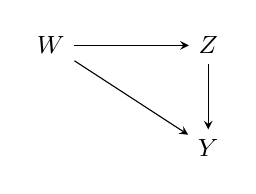
\begin{tikzpicture}[>=stealth,every node/.style={font=\small}]
\node (w) at (0,1) {$W$}; \node (z) at (2,1) {$Z$}; \node (y) at (2,-.3) {$Y$};
\draw[->] (w)--(z); \draw[->] (z)--(y); \draw[->] (w)--(y);
\end{tikzpicture}
\end{center}
原稿接着写道
\[
 P[Y\mid\operatorname{do}(W=0),\operatorname{do}(Z=Z(w=1))]
 =f_Y\bigl(w=0,z=f_Z(w=1,\varepsilon_Z),\varepsilon_Y\bigr).
\]
\inkred{不同的潜在设置可以放在一起讨论；Potential Outcome 中不行，除非作图？}
\begin{reviewnote}{original}{S2-022}{反事实变量不等于它的分布}{Lecture11-14.pdf, page 22}
两边类型一致的等式应为
\[
 Y(0,Z(1))=f_Y(0,f_Z(1,\varepsilon_Z),\varepsilon_Y).
\]
其分布是 $\mathcal L(Y(0,Z(1)))$，而不是随机变量本身。手写等式和官方讲义对应的例子都存在这种类型不匹配。
\end{reviewnote}


\textbf{笔记记录的一些观点：}SEM 可以识别上述操作的因果效应，被一些人认为是 SEM 的缺陷；潜在结果表述不能识别，则被认为是其局限性。\notearrow{red}{可识别？}{SEM 能识别这种嵌套操作的说法。}这里记录的是疑问和观点，并非由翻译替作者作出的定论。

\begin{reviewnote}{original}{S2-023}{潜在结果也能表达嵌套反事实}{Lecture11-14.pdf, page 22}
关于记号局限性的说法不正确：$Y(0,Z(1))$ 恰好表达了这一嵌套量。任何一种记号本身都不能证明识别。关于中介分析中的嵌套潜在结果，参见 \href{https://imai.sites.fas.harvard.edu/research/files/BaronKenny.pdf}{Imai、Keele 和 Tingley（2010）}。
\end{reviewnote}

\begin{reviewnote}{qualification}{S2-024}{回答页边疑问：需要哪些识别假设？}{Lecture11-14.pdf, page 22}
对图中所有节点均可观测、结构误差相互独立且支持充分的情形，
\[
 E[Y(0,Z(1))]=\int E[Y\mid W=0,Z=z]\,dP(Z=z\mid W=1).
\]
SEM 提供了相关的跨世界独立性。若中介与结果之间有潜在混杂，或仅作更弱的单世界假设，这个公式就可能不成立。因此，红字“可识别？”提出的是实质性的模型问题。\href{https://imai.sites.fas.harvard.edu/research/files/BaronKenny.pdf}{Imai 等人} 区分了定义与识别。
\end{reviewnote}


\section{第 14 讲：自适应实验}
\sourcepages{Lecture11-14.pdf, page 24, with the explanatory note on page 23}
自适应实验动态调整实验设计。此前的固定实验在 IID 框架下进行，而这一假设有时过于严格。

\subsection{设定与记号}
有动作 $k=1,\ldots,K$ 和受试者 $t=1,\ldots,T$。不同受试者的潜在结果独立同分布。记
\[
 Y_t(k)\sim F_k,\qquad Y_t=Y_t(W_t),\qquad
 \mu_k=\mathbb E[Y_t(k)].
\]
$W_t$ 是为第 $t$ 个受试者选择的动作，$F_k$ 是臂 $k$ 的潜在结果分布，$\mu_k$ 是其均值。定义 regret：
\[
 R_T=\sum_{t=1}^T(\mu^*-\mu_{W_t}),\qquad
 \mu^*=\sup_{1\le k\le K}\mu_k.
\]
$\mu^*$ 是所有可用动作中最大的期望奖励。Regret 衡量：相较于始终选择最优动作，选择当前动作序列损失了多少期望奖励。

定义
\[
 n_{kt}=\sum_{j=1}^t\mathbf1\{W_j=k\},\qquad
 \widehat\mu_{kt}=\frac1{n_{kt}}\sum_{j=1}^t\mathbf1\{W_j=k\}Y_j.
\]
\notearrow{black}{$n_{kt}$}{截至时点 $t$，选择臂 $k$ 的次数。}
\notearrow{black}{$\widehat\mu_{kt}$}{臂 $k$ 的平均奖励。}
\inkred{使用的是从第 $1$ 期到第 $t$ 期收集的信息。}

\paragraph{我在左页的重新表述。}
可以想象有 $T$ 个相似、独立的个体。每个人都有 $K$ 种处理选择，因而有 $K$ 个潜在结果，各臂对应的分布 $F_k$ 对所有人相同。对每个人，只能观测被选择处理的结果 $Y_t=Y_t(W_t)$。向量 $\mu$ 收集了各臂的期望奖励。总 regret 就是对 $T$ 个人累加：所选处理与最优处理之间的差距；在这个设定中，最优臂始终是同一个。

在普通随机实验中，$W_t$ 在 $1,\ldots,K$ 上均匀且非自适应地选择，因此 regret 随 $T$ 线性增长：
\[
 R_T\sim T\sum_{k=1}^K\frac{\mu^*-\mu_k}{K}.
\]
\inkblue{批注把求和项的平均解释为每个个体的期望损失。}自适应实验的首要目标是使 regret 次线性增长。\notearrow{red}{Regret 不应随实验次数或时间线性增长；选择要逐渐接近最优。}{次线性 regret。}这需要平衡\emph{探索}（尝试）与\emph{利用}（使用已有知识）。

\subsection{面对不确定性时保持乐观}
\sourcepages{Lecture11-14.pdf, page 25}
置信上界（UCB）方法平衡探索与利用：
\begin{enumerate}
 \item 对每个臂抽样 $t_0$ 次进行初始化：\inkred{选择并观测 $t_0$ 次，一共 $Kt_0$ 次初始抽样。}
 \item 对每个 $t=Kt_0+1,Kt_0+2,\ldots$，基于截至 $t-1$ 收集的数据，为每个 $\mu_k$ 构造置信区间 $\widehat U_{kt}$。
 \item 选择置信区间上端点最大的动作 $W_t$，观测 $Y_t=Y_t(W_t)$。
\end{enumerate}
\inkred{每过一个 $t$，只多了一个数据点。}

为理解 UCB 控制 regret 的原理，将奖励简化为高斯分布：
\[
 Y_t(k)\sim\mathcal N(\mu_k,b^2),\tag{14.4}
\]
其中 $b^2$ 已知。\notearrow{blue}{这里已知是为了简化计算。}{高斯 UCB 半径中的 $b^2$。}使用
\[
 \widehat U_{kt}=\widehat\mu_{k,t-1}
 \ \pm\ b\sqrt{\frac{4\log T}{n_{k,t-1}}}.\tag{14.5}
\]
当 $t_0=1$ 时，笔记给出的 regret 表达式为
\[
 R_T=\sum_{k\ne k^*}
 \left\{\frac{16b^2\log T}{\mu_{k^*}-\mu_k}
 +(\mu_{k^*}-\mu_k)\right\},\tag{14.6}
\]
以至少 $1-K/T$ 的概率成立，其中 $k^*$ 表示最优臂。

\begin{reviewnote}{original}{S2-025}{UCB 的 regret 结论是上界}{Lecture11-14.pdf, pages 25, 27, 28}
应将 (14.6)、第 27 页重写的结论以及第 28 页最后一个式子中的 $=$ 改为 $\le$。对 $\Delta_k=\mu^*-\mu_k>0$，证明给出的是 $n_{kT}\le16b^2\log T/\Delta_k^2+1$，而不是等式。求和只应包含严格次优的臂；并列最优的臂 regret 为零，不能把它们放进分母为零的项。官方讲义也重复了这个等号笔误。
\end{reviewnote}


\paragraph{我对这个界的直觉。}
\notearrow{red}{分母中的差距 $\mu_{k^*}-\mu_k$。}{\inkred{臂与最优臂越接近，UCB 越需要更长的时间分辨；很差的臂可快速丢弃。}}

\inkred{UCB 的 regret 只以对数增长。臂与最优臂越接近，越需要更长时间分辨；很差的臂可以快速丢弃。$\mu_{k^*}-\mu_k$ 很小时，看起来会使上面的界趋向无穷。实际上有两个相互竞争的界：effect 强时，UCB 在置信区间分离后丢弃该臂；effect 弱时，总 regret 至多为 $T(\mu_{k^*}-\mu_k)$。结合两者就得到有限上界；即使对所有均值取最坏情况，笔记仍给出了 $K\sqrt{T\log T}$ 阶的上界。}续页的两幅草图比较了增长速度（重绘如下）。

\begin{reviewnote}{original}{S2-026}{一致最坏情形界不能允许均值差无界}{Lecture11-14.pdf, page 25}
声称对所有实数均值都成立的一致上界不正确：初始化时每个臂各选一次，就已经付出了 $\sum_k\Delta_k$，该量可以无界。在置信事件上，
\[
 R_T\le\sum_{k:\Delta_k>0}\min\left\{T\Delta_k,\frac{16b^2\log T}{\Delta_k}+\Delta_k\right\}.
\]
若均值差一致有界且 $b$ 固定，强／弱效应比较可以给出所述 $O(K\sqrt{T\log T})$ 量级，再加初始化代价。补上这个限制后，原直觉才成立。
\end{reviewnote}


\subsection{UCB 的 regret 上界}
\sourcepages{Lecture11-14.pdf, page 27, with the attempted concentration calculation on page 26, then page 28}
将 regret 改写为
\[
 R_T=\sum_{k\ne k^*}n_{kT}(\mu_{k^*}-\mu_k).
\]
主要任务是控制 $n_{kT}$，即 UCB 选择次优臂的次数。\notearrow{red}{这也是 UCB 的设计原理。}{控制次优臂的选择次数 $n_{kT}$。}

设 $\zeta_{kj}$ 是臂 $k$ 第 $j$ 次被选择的时间。对 $t=K+1,\ldots,T$，笔记推导以下概率界：
\begin{align*}
 &P\left[\sup_{K<t\le T}\left\{
 \mu_k-\widehat\mu_{k,t-1}
 -b\sqrt{\frac{4\log T}{n_{k,t-1}}}\right\}\ge0\right]\\
 &\quad\le P\left[\sup_{1\le j\le n_{kT}}\left\{
 \mu_k-\widehat\mu_{k,\zeta_{kj}}
 -b\sqrt{\frac{4\log T}{j}}\right\}\ge0\right]\\
 &\quad=P\left[\sup_{1\le j\le n_{kT}}\left\{
 \mu_k-\frac1j\sum_{\ell=1}^jY'_\ell(k)
 -b\sqrt{\frac{4\log T}{j}}\right\}\ge0\right]\\
 &\quad\le P\left[\sup_{1\le j\le T}\left\{
 \mu_k-\frac1j\sum_{\ell=1}^jY'_\ell(k)
 -b\sqrt{\frac{4\log T}{j}}\right\}\ge0\right]
 \le\frac1T.
\end{align*}
其中 $Y'_\ell(k)$ 是从 $\mathcal N(\mu_k,b^2)$ 独立抽取的观测。\notearrow{red}{扩大索引集合，上确界及相应事件只会变大；奖励序列的分布相同。}{$K<t\le T\ \leadsto\ 1\le j\le n_{kT}\ \leadsto\ 1\le j\le T$}
对应的两行手写式使用的是 $Y'_\ell(0)$。
\begin{reviewnote}{original}{S2-027}{时间变换后的观测仍属于臂 k}{Lecture11-14.pdf, page 27}
这两处都应为 $Y'_\ell(k)$，如所展示的推导。可以预先为每个臂生成一列 IID 奖励，每次选中该臂时，揭示其中的下一个观测。对确定的计数 $j\le T$ 使用 union bound，可避免错误地认为给定随机样本量后，停止采样的样本均值仍由条件 IID 观测构成。
\end{reviewnote}


因此，对每个臂 $k$，以至少 $1-1/T$ 的概率，
\[
 \mu_k\le\widehat\mu_{k,t-1}
 +b\sqrt{\frac{4\log T}{n_{k,t-1}}}
 \quad\text{对所有 }t=K+1,\ldots,T.\tag{14.8}
\]
再对 $K$ 个臂取 union bound，就得到至少 $1-K/T$ 的概率。

\paragraph{左页推算：Hoeffding 不等式，以及我尚未解决的计算。}
对相互独立的有界随机变量 $Z_1,\ldots,Z_n$，若几乎必然有 $Z_i\in[a,b]$，且 $s>0$，则
\[
 P\left(\frac1n\sum_{i=1}^n(Z_i-\mathbb E[Z_i])\ge s\right)
 \le\exp\left(-\frac{2ns^2}{(b-a)^2}\right).
\]
下尾偏差 $\le-s$ 也满足同样的界；双侧绝对偏差的界多一个因子 $2$。\notearrow{red}{几乎肯定有界。}{$Z_i\in[a,b]$}

对事件 $A_1,\ldots,A_n$，union bound 为
\[
 P(A_1\cup\cdots\cup A_n)\le\sum_{i=1}^nP(A_i).
\]
笔记将它与 $1-K/T$ 的保证联系起来。

\textbf{我的计算尝试（保留尚未解决的疑问）：}猜吧，只需证明
\[
 P\left(\mu_k-\frac1j\sum_{\ell=1}^jY'_\ell(k)
 -b\sqrt{\frac{4\log T}{j}}\ge0\right)\le\frac1T.
\]
而左边为
\[
 P\left(\frac1j\sum_{\ell=1}^jY'_\ell(k)-\mu_k
 \le-b\sqrt{\frac{4\log T}{j}}\right).
\]
套用上面针对有界变量的不等式，似乎会得到
\[
 \exp\left(-\frac{2j\,b^2(4\log T)/j}{(b-a)^2}\right)
 =\exp\left(-\frac{8b^2}{(b-a)^2}\log T\right)
 \le\frac1T.
\]
\inkred{\textbf{作者的红字疑问：}“$Y'_\ell(k)$ 无界，$k$ 是否写错了？”以及“不知道怎么化的，可能有未说明的假设。”}

\begin{reviewnote}{qualification}{S2-028}{补完尚未完成的高斯尾概率计算}{Lecture11-14.pdf, pages 26, 27}
作者的红字质疑是对的：有界变量的 Hoeffding 不等式不能用于这里。应改用
\[
 \sqrt j(\overline Y'_{kj}-\mu_k)/b\sim N(0,1),
\]
\[
 P\left(|\overline Y'_{kj}-\mu_k|>b\sqrt{4\log T/j}\right)
 =2\Phi(-2\sqrt{\log T})\le T^{-2}\quad(T\ge2).
\]
最后一步来自正态分布的 Mills 界 $2\Phi(-x)\le2e^{-x^2/2}/(x\sqrt{2\pi})$。对至多 $KT$ 个“臂／计数”组合取 union bound，可得至少 $1-K/T$ 的同时双侧覆盖概率。若每个计数只有 $1/T$ 的界，再对 $T$ 个计数取并集就不够了。这些是补充的证明细节，并非原扫描已有的陈述。字母 $b$ 在两处代表的不同含义也不应混淆。
\end{reviewnote}


\paragraph{继续推导臂的选择次数界。}
若 (14.8) 对所有臂都成立，且 $W_t=k$，则由 UCB 的选择规则，
\begin{align*}
 \widehat\mu_{k,t-1}+b\sqrt{\frac{4\log T}{n_{k,t-1}}}
 &\ge\widehat\mu_{k^*,t-1}+b\sqrt{\frac{4\log T}{n_{k^*,t-1}}}\\
 &\ge\mu_{k^*}.
\end{align*}
笔记接着写道
\[
 \mu_k+2b\sqrt{\frac{4\log T}{n_{k,t-1}}}\ge\mu_{k^*},
 \qquad
 n_{k,t-1}\le\frac{16b^2\log T}{(\mu_{k^*}-\mu_k)^2}.
\]
\notearrow{red}{置信结论（1），然后 UCB 选择 $k$。}{次数界（2）：$n_{k,t-1}\le16b^2\log T/\Delta_k^2$。}

\begin{reviewnote}{original}{S2-029}{次数界还需要另一方向的偏差控制}{Lecture11-14.pdf, pages 27, 28}
仅有 (14.8) 不足以推出这一步。记 $r_{kt}=b\sqrt{4\log T/n_{k,t-1}}$。在前面所述双侧事件上，选择 $k$ 意味着
\[
 \mu^*\le\widehat\mu_{k^*,t-1}+r_{k^*t}
 \le\widehat\mu_{k,t-1}+r_{kt}\le\mu_k+2r_{kt}.
\]
最后一步需要 $\widehat\mu_{k,t-1}-\mu_k\le r_{kt}$，这正是遗漏的偏差方向。平方后即可得到次数阈值。使用相同的高斯置信常数可以补全定理，但手写证明本身不完整。
\end{reviewnote}


\inkred{\textbf{我的理解：}选择臂 $k$，说明它的置信区间上端点还必须高于最优臂的上端点。一旦选择次数超过阈值，而阈值只随 $\log T$ 增长，在这个论证中就不能再选择它了。}

把次数上界代入 regret 的定义：
\begin{center}
\begin{tikzpicture}[>=stealth,red,every node/.style={font=\scriptsize}]
\draw[->] (0,0)--(3,0); \draw[->] (0,0)--(0,1.7);
\draw (0,0)--(2.4,1.5); \draw (0,0) .. controls (.5,.65) and (1.5,.8) .. (2.7,.9);
\node at (1.5,-.35) {增长速度的定性比较};
\begin{scope}[xshift=5cm]
\draw[->] (0,0)--(3,0); \draw[->] (0,0)--(0,1.7);
\draw (0,.7)--(2.8,.7); \draw (.1,-.1) .. controls (.5,1.4) and (1.7,1.5) .. (2.7,1.55);
\node at (1.5,-.35) {越过阈值};
\end{scope}
\end{tikzpicture}
\end{center}
\[
 R_T=\sum_{k\ne k^*}(\mu_{k^*}-\mu_k)n_{kT}
 \ =\ \sum_{k\ne k^*}\left\{
 \frac{16b^2\log T}{\mu_{k^*}-\mu_k}+(\mu_{k^*}-\mu_k)\right\}.
\]
\inkred{最后加上的均值差，是该臂初始化时 $t_0=1$ 次选择带来的 regret；第一项对应 $t=K+1,\ldots,T$。}等号按扫描原样保留；前面的紫色上界校注也适用于这里。

\subsection{自适应随机化方案}
\sourcepages{Lecture11-14.pdf, page 29}
UCB 有局限：难以与为 IID 采样开发的方法结合，也难以推广到更复杂的采样设计。例如，不同臂的不确定性可能不同，在更一般的设计中，构造可比较的区间 $\widehat U_{kt}$ 会比较麻烦 [手写括号内部分不清楚]。\inkred{红字将 UCB 对历史观测的依赖，与基于随机 IID 数据的方法作对比 [最右边括号中的简短批注不清楚]。}

\paragraph{Thompson 采样。}
这是 UCB 的替代方案：\inkred{基于 Bayesian 更新的启发式算法。}
\begin{enumerate}
 \item 为每个潜在结果分布 $F_k$ 选择先验 $\Pi_{k,0}$。
 \item 在时点 $t$，计算臂 $k$ 是最优臂的后验概率：
 \[e_{k,t-1}=P_{\Pi_{t-1}}(\mu_k=\mu^*).\]
 \item 随机选择动作：
 \[W_t\sim\operatorname{Multinomial}(e_{\cdot,t-1}).\]
 \item 观测 $Y_t=Y_t(W_t)$，并将后验更新为 $\Pi_t$。
\end{enumerate}
Thompson 采样与 UCB 有相似的统计行为：周期性地对每个臂采样，直到基本确信该臂较差。\notearrow{red}{后验概率降到 $1/T$ 以下。}{基本确信该臂较差。}

\begin{reviewnote}{qualification}{S2-031}{并列最优臂与 Thompson 的启发式解释}{Lecture11-14.pdf, page 29}
若后验下的最优臂几乎必然唯一，各臂最优的概率才直接加和为一；否则需要规定打破平局的规则。这里的 $\operatorname{Multinomial}$ 指一次分类抽样。概率降到 $1/T$ 以下，是对剩余被选概率可忽略的直觉说明，不是算法强制设置的截断点。UCB 与 Thompson 具有相似 regret 行为，还需要相应的模型、先验及正则条件。
\end{reviewnote}


Thompson 采样中的动作是随机的，自适应随机化概率依赖过去的数据。这自然可以与因果推断结合。
\notearrow{black}{Thompson 采样使用依赖历史数据的概率随机选择动作。}{与因果推断结合。}笔记指出，调整先验 $\Pi_0$ 可能比调整 UCB 区间 $\widehat U_{kt}$ 更合理。

\subsection{自适应实验中的统计推断}
\sourcepages{Lecture11-14.pdf, page 31, with the derivation on page 30}
分析由 UCB 或 Thompson 采样得到的数据，并对问题背后的参数给出置信结论。这比 IID 情形困难得多。

$\mu_k$ 的两个自然估计量，一是样本均值：
\[
 \widehat\mu_k^{\mathrm{AVG}}=\widehat\mu_{kT}
 =\frac1{n_{kT}}\sum_{t=1}^T\mathbf1\{W_t=k\}Y_t,\tag{14.11}
\]
二是 Thompson 采样下的 IPW 估计量：

\begin{reviewnote}{qualification}{S2-033}{使用观测当前结果之前的分配概率}{Lecture11-14.pdf, pages 29, 31}
定义 $e_{tk}=P(W_t=k\mid\mathcal H_{t-1})$，在第 $t$ 个受试者的结果出现之前计算；它就是前面的 $e_{k,t-1}$。需要正性条件。通常的确定性 UCB 给出的条件概率是 $0$ 或 $1$，因此这些 IPW／AW 公式不能直接用于其未选择的臂。样本均值还要求 $n_{kT}>0$。
\end{reviewnote}

\[
 \widehat\mu_k^{\mathrm{IPW}}=\frac1T\sum_{t=1}^T
 \frac{\mathbf1\{W_t=k\}Y_t}{e_{tk}}.\tag{14.12}
\]
由于数据收集是自适应的，这些估计量没有渐近正态极限分布，所以置信区间难以构造。
\begin{reviewnote}{original}{S2-032}{自适应性并不排除所有正态极限}{Lecture11-14.pdf, page 31}
正确的提醒是：在不加限制的自适应设计下，这些估计量\emph{未必}具有正态极限。固定的正分配概率适用普通 CLT；经过适当稳定化的自适应设计也可能满足 CLT。正的可预测概率仍可使固定终点下、未归一化的 IPW 均值保持无偏，但无偏并不蕴含正态性。参见 \href{https://pmc.ncbi.nlm.nih.gov/articles/PMC8054003/}{Hadad 等（2021）}。
\end{reviewnote}


自适应加权估计量可以得到高斯枢轴量：
\inkred{高斯枢轴量接近，或依分布收敛到 $N(0,1)$。}
\[
 \widehat\mu_k^{\mathrm{AW}}
 =\frac{\displaystyle\sum_{t=1}^T
 \frac{\mathbf1\{W_t=k\}Y_t}{\sqrt{e_{tk}}}}
 {\displaystyle\sum_{t=1}^T
 \frac{\mathbf1\{W_t=k\}}{\sqrt{e_{tk}}}}.\tag{14.13}
\]
在合理的正则条件下，
\[
 \widehat V_k^{-1/2}(\widehat\mu_k^{\mathrm{AW}}-\mu_k)
 \ \Rightarrow\ \mathcal N(0,1),
\]
其中
\[
 \widehat V_k=
 \frac{\displaystyle\sum_{t=1}^T
 \left\{\frac{\mathbf1\{W_t=k\}(Y_t-\widehat\mu_k^{\mathrm{AW}})}
 {\sqrt{e_{tk}}}\right\}^{\!2}}
 {\displaystyle\left\{\sum_{t=1}^T
 \frac{\mathbf1\{W_t=k\}}{\sqrt{e_{tk}}}\right\}^{\!2}}.\tag{14.14}
\]
\textbf{我的解释：}由于估计量稳定了方差，便可以恢复 CLT。它的方差变得可控制，从而能应用中心极限定理。

\paragraph{左页推导：估计量背后的鞅。}
页顶先给出了鞅的定义：变量对可用历史可测，满足 $\mathbb E[X_i]<\infty$，并满足条件均值恒等式。另一行将适应过程 $M_n$ 描述为只依赖 $X_0,\ldots,X_n$，且
$\mathbb E[M_n\mid X_0,\ldots,X_{n-1}]=M_{n-1}$.

\begin{reviewnote}{original}{S2-034}{鞅的可积性应使用绝对矩}{Lecture11-14.pdf, page 30}
应写 $E|X_i|<\infty$。仅有单侧不等式 $E[X_i]<\infty$ 可能容许 $-\infty$，不能保证所需的条件期望存在。如果“有限期望”本意是有限实数期望，则已经隐含可积性；加上绝对值可将它明确写出。
\end{reviewnote}


由 (14.13)，
\[
 \widehat\mu_k^{\mathrm{AW}}-\mu_k
 =\frac{\displaystyle\sum_{t=1}^T
 \frac{\mathbf1\{W_t=k\}(Y_t-\mu_k)}{\sqrt{e_{tk}}}}
 {\displaystyle\sum_{t=1}^T
 \frac{\mathbf1\{W_t=k\}}{\sqrt{e_{tk}}}}.
\]
令分子中的部分和为
\[
 M_t=\sum_{j=1}^t
 \frac{\mathbf1\{W_j=k\}(Y_j-\mu_k)}{\sqrt{e_{jk}}}.
\]
$W_t$ 根据截至时点 $t$ 可用的信息随机选择，并且给定过去后与 $Y_t(k)$ 独立。因此，$M_t$ 是鞅：
\[
 \mathbb E[M_t\mid M_1,\ldots,M_{t-1}]=M_{t-1}.
\]
\inkred{红字重新写为 $\mathbb E[M_{t+1}\mid M_1,\ldots,M_t]=M_t$。}

原稿接着写：“由加权方案”，
\[
 \operatorname{Var}[M_t\mid M_1,\ldots,M_{t-1}]=b_k^2,
 \qquad b_k^2=\operatorname{Var}[Y_t(k)].\tag{14.8，原稿标号}
\]
给定之前的部分和后，这也就是新增加一项的条件方差。笔记重复使用了编号 (14.8)。

只要 $e_{tk}$ 不衰减得太快，由鞅 CLT 可得
\[
 \frac{M_T}{\sqrt{Tb_k^2}}\Rightarrow\mathcal N(0,1).
\]
\inkred{\textbf{作者的红字批注：}自适应加权的 CLT；有限二阶矩；抽样概率 $e_{tk}$ 的衰减速度应慢于 $1/t$。这排除了最激进的强有效探索方案：一个臂只抽样 $\log T$ 量级的次数。}

\begin{reviewnote}{qualification}{S2-035}{鞅枢轴量的一组充分条件}{Lecture11-14.pdf, pages 30, 31}
一组清楚的充分条件是：$0<b_k^2<\infty$，$E|Y_t(k)-\mu_k|^4<\infty$，可预测的 $e_{tk}\ge c t^{-\alpha}$，其中 $c>0$、$0\le\alpha<1$，且当前潜在结果独立于过去的数据。对 $D_t=\mathbf1\{W_t=k\}(Y_t-\mu_k)/\sqrt{e_{tk}}$，
\[
 E[D_t\mid\mathcal H_{t-1}]=0,\quad E[D_t^2\mid\mathcal H_{t-1}]=b_k^2,\quad
 T^{-2}\sum_{t\le T}E[D_t^4]=O(T^{\alpha-1})\to0.
\]
由此得到鞅 Lyapunov 条件，以及 $T^{-1}\sum D_t^2$ 的集中性。AW 分母的可预测均值量级至少为 $T^{1-\alpha/2}$，波动为 $O_P(\sqrt T)$，因此可得一致性，并允许在方差中使用拟合残差。这些条件充分但非必要。原稿的 $\operatorname{Var}(M_t\mid M_{1:t-1})=b_k^2$ 在这里是正确的：$M_{t-1}$ 已知，而新增一项具有该方差。更一般的条件见 \href{https://pmc.ncbi.nlm.nih.gov/articles/PMC8054003/}{Hadad 等（2021）}。
\end{reviewnote}


接着，
\[
 \frac1{Tb_k^2}\sum_{t=1}^T
 \left\{\frac{\mathbf1\{W_t=k\}(Y_t-\widehat\mu_k^{\mathrm{AW}})}
 {\sqrt{e_{tk}}}\right\}^{\!2}
 \xrightarrow{P}1.
\]
这一步证明集中性；页边再次要求概率不要衰减得太快。$\widehat\mu_k^{\mathrm{AW}}-\mu_k$ 与 $\widehat V_k^{1/2}$ 的分母相消，就得到前面的高斯枢轴量。
\notearrow{black}{$\widehat\mu_k^{\mathrm{AW}}-\mu_k$ 与 $\widehat V_k^{1/2}$ 的分母相消。}{式 (14.14) 中的高斯枢轴量。}
